\documentclass[conference]{IEEEtran}
\IEEEoverridecommandlockouts
% The preceding line is only needed to identify funding in the first footnote. If that is unneeded, please comment it out.
\usepackage{cite}
\usepackage{amsmath,amssymb,amsfonts}
\usepackage{algorithmic}
\usepackage{graphicx}
\usepackage{textcomp}
\usepackage{xcolor}
\usepackage{subcaption}
\usepackage{extarrows}

\def\BibTeX{{\rm B\kern-.05em{\sc i\kern-.025em b}\kern-.08em
    T\kern-.1667em\lower.7ex\hbox{E}\kern-.125emX}}
\begin{document}

\title{ECE276A PR2 Report}

\author{
\IEEEauthorblockN{1\textsuperscript{st} Weixiao Zhan}
\IEEEauthorblockA{
    weixiao-zhan[at]ucsd[dot]edu}
}

\maketitle


\section{Introduction}
Simultaneous Localization and Mapping (SLAM) is pivotal in robotics, 
enabling autonomous systems to understand their surroundings and their locations 
with minimal human intervention. 
In this project, SLAM on a differential-drive robot equipped with a wheel encoder, 
an Inertial Measurement Unit (IMU), 2-D LiDAR, and an RGBD camera is implemented,
which optimize the robot trajectory,  
and reconstructed detailed occupancy and floor texture map.

The process began with the construction of a motion model trajectory based on 
the differential-drive kinematics, 
utilizing data from the wheel encoder and IMU. 
Concurrently, an observation model trajectory was estimated using LiDAR scans 
and the Iterative Closest Points (ICP) method. 
Subsequently, I applied a Factor Graph and loop closure techniques to 
refine and optimize the trajectory. 
Lastly, I leveraged the trajectories to generate 
detailed maps, showcasing the potential.


\section{Problem Formulation}
The robot trajectory, discretized as a set of pose and time stamp tuples, 
is the core of computation.
Denote the robot's pose at given time stamp \(t\) as \(P_t\).
The pose can be represented in both two-dimensional (2D) and three-dimensional (3D) spaces, 
with the z-axis value fixed at zero. 
$$
P_{t} = \begin{cases}
    \xlongequal{2D} \left[ \begin{gathered}x\\ y\\ \theta \end{gathered} \right] & \in \mathbb{R}^{3} \\ 
    \xlongequal{3D} \left[ \begin{matrix}R_{yaw}(\theta )&\left[ \begin{gathered}x\\ y\\0\end{gathered} \right]  \\ \mathbf{0}&1\end{matrix} \right] & \in \mathbb{R}^{[4\times 4]}
\end{cases} 
$$
These representations imply the same intrinsics 
and will be used seamlessly in following 2D-3D-mixed analysis.
The initial pose $P_0$ at time 0 is also defined as the world frame
serving as the reference for all subsequent poses.
$$P_{0}=\begin{cases}\vec{0}_{3}\\ I_{4}\end{cases} $$

\subsection{Motion Model: IMU \& Differential-drive Kinematics}
Consider a small time interval $\tau$ between two consecutive time stamp $t-1$ and $t$.
Suppose wheel encoder and IMU reports the robot has traveled $\delta d$ ($m$) distance and 
and rotated $\delta \theta$ (rad) during this interval,
the motion of robot can be approximate as an arc:
$$
\begin{aligned}
    {}_{t-1}O_{t}
        & =\left[ \begin{gathered}\delta d\cdot \mathrm{sinc} \left( \frac{\delta \theta }{2} \right)  \sin \left( \theta_{t} +\frac{\delta \theta }{2} \right)  \\ \delta d\cdot \mathrm{sinc} \left( \frac{\delta \theta }{2} \right)  \sin \left( \theta_{t} +\frac{\delta \theta }{2} \right)  \\ \delta \theta \end{gathered} \right] \\
    P_{t}^{(2M)}
    &=P_{0}^{(2M)} + \sum_{f=1}^{t} {}_{f-1}O_{f}
\end{aligned} 
$$
in which, the superscript $^{(2M)}$ means this is a 2D motion model trajectory,


\subsection{Observation Model: LiDAR \& Scan Matching}
Scan matching can, given observations at different poses,
estimate their elative transformations.
Scan matching on LiDAR scan is used as observation model in this project.

2D-LiDAR scan reports a set of range and angle tuple $L_t = \{(r_i, \phi_i)\}$ at time stamp $t$,
which can be converted to a set of 3D point cloud in body frame using following equations:
$$
\begin{aligned}
    \mathrm{PC}_{\text{LiDAR frame}} 
        &= \left\{ \left[ \begin{gathered}r_i\sin \phi_i \\ r_i\cos \phi_i \\ 0\end{gathered} \right] \bigg| \forall (r_i, \phi_i)\in L_t\right\} 
        \\
    \left[ \begin{gathered} \mathrm{PC}_t \\ 1\end{gathered} \right]  
    &= _{\text{body}}T_{\text{LiDAR}}  \left[ \begin{gathered} \mathrm{PC}_{\text{LiDAR frame}}  \\ 1\end{gathered} \right]  
\end{aligned}
$$

Since there is  prior knowledge of data association between two LiDAR scans,
ICP algorithm is used.
Given two homogenous point clouds, 
source $S = \left\{\left[ \begin{matrix}PC_{s}& 1\end{matrix} \right]^T \right\} $ at timestamp $s$,
and target $T = \left\{\left[ \begin{matrix}PC_{t}& 1\end{matrix} \right]^T \right\}$ at timestamp $t$,
and an initial guess transformation $T_0$,
ICP iterates following steps:
\begin{enumerate}
    \item Apply initial guess: $S \leftarrow T_0 \cdot S$ and set $k \leftarrow 1$.
    
    \item Find point association using nearest neighbor:
    $$ \Delta = \left\{\left(s, \arg\min_{t\in T} \|s - t\| \right) \bigg| \forall s\in S\right\}$$

    \item Estimate relative transformation $T_k$ using Kabsch algorithm:
    $$T_k = \arg\min_{T\in SE(3)} \sum\limits_{(s,t)\in\Delta} \|t - Ts\|$$.
    
    \item Update $S \leftarrow T_k \cdot S$, increase $k$ by 1, and repeat from step 2 until no improvement.

    \item Compose and return the total transformation and error 
    $$ \begin{aligned}
        {}_tT_s & = \prod_k T_k \\
        {}_t\epsilon_s &= \frac{1}{|\Delta|} \sum_{(s,t)\in\Delta} \|t - {}_tT_s\cdot s\| 
    \end{aligned}$$
\end{enumerate}


Using ICP to estimate relative transformation between consecutive LiDAR scans,
observation model trajectory is composed as following:
$$
\begin{aligned}
    _{t-1}T_{t}
        &=\text{ICP}(S=\mathrm{PC}_{t}, T=\mathrm{PC}_{t-1}) \\ 
    P^{(3O)}_{t}
        &=P_{0}\prod^{t}_{f=1} {}_{f-1}T_{f} = {}_{0}T_{t}
\end{aligned} 
$$
in which, the superscript $^{(3O)}$ means this is a 3D observation trajectory.

\subsection{Factor Graph and Loop Closure}
Factor graph is a constrained optimization model for SLAM problem.
Graph nodes represent robot states as random variables,
while edges represent motion and observation constraints as conditional distributions.
The optimizer of a factor graph is the random variables that maximize likelihood of all factors.

Loop Closure is a special type of constraint in factor graph.
Typical constraints based on Markov assumption builds a single chain graph, 
in which error and noise accumulate.
However, when some temporally distant robot states are spatially close,
it is possible to estimate their relative transformations,
thereby create loops in factor graph and reduce accumulated error.

A loop detection criteria based on max location difference $d^*$, 
max yaw difference $\theta^*$, and min interval $\tau^*$
is used to find potential loop closure pose pairs $lc$:
$$
lc = \left\{(i, j) \bigg| 
\begin{aligned}
    \| P_{i}[xy]-P_{j}[xy]\| &< d^*\\ 
    \| P_{i}[\theta]-P_{j}[\theta]\| &< \theta^* \\
    |i-j|&>\tau^*
\end{aligned} 
, \forall i, j\right\}
$$

The factor graph is construct as:
$$
\begin{aligned}
G &= (V, E) \\
V &= \{ P_{t},\ \forall t\} \\
E &= \left\{ \begin{gathered}
\underbrace{P_{t}^{(2)} \ominus \left(P_{t-1}^{(2)} + {}_{t-1}O_{t} \right),\forall t}_{\text{motion constraints}} \\
\underbrace{P_{t}^{(3)} \ominus \left(P_{t-1}^{(3)} \cdot {}_{t-1}T_{t} \right),\forall t}_{\text{observation constraints}} \\
\underbrace{\begin{gathered} P_{i}^{(3)} \ominus \left(P_{j}^{(3)} \cdot \text{ICP}(S=\mathrm{PC}_{i}, T=\mathrm{PC}_{j}) \right) \\ \forall (i,j) \in lc \end{gathered}}_{\text{loop closure constraints}}
\end{gathered} \right\}
\end{aligned}
$$
The three types of constraints are:
\begin{enumerate}
\item Motion constraints applied to two consecutive poses, derived differential drive kinematics.
\item Observation constraints on two consecutive poses, utilizing scan matching (ICP).
\item Loop closure constraints on poses that are spatially proximate yet temporally distant.
\end{enumerate}


\subsection{Mapping}
Mapping is another critical component of SLAM, 
which reconstructs the surrounding environment using various sensors.
2D LiDAR was used to construct an occupancy map, 
while an RGB-D camera, which provides both RGB and disparity information,
was employed for texture mapping of the environment.

\subsubsection{Occupancy}
LiDAR scan $(r_i, \phi_i)$ infer that 
the end-points ($\{(r_i\cos\phi_i, r_i\sin\phi_i), \forall i\}$ in LiDAR frame) are occupied,
while the space between the end-points and LiDAR sensor origin 
($(0, 0)$ in LiDAR frame) and is empty.

By transforming the endpoints and LiDAR sensor to world frame,
discretizing the world floor into a grid of cells,
using Bresenham ray tracing to obtain empty and occupied cell set,
the probability of occupancy of each cells can be estimate by
logistic regression over all scans.

\subsubsection{RGB Texture}
Consider values $d$ at pixel $(u, v)$ of the disparity image 
and its associated $rgb$ value.
Given the intrinsic matrix $K$ of the D camera, 
the equations to convert disparity value $d$ to the associated depth $z$,
and the projection equation:
$$
\begin{aligned}
    z&=g(d)\\ 
    \left[ \begin{gathered}u\\ v\end{gathered} \right]  &=K\pi \left( \left[ \begin{gathered}x\\ y\\ z\end{gathered} \right]_{opt}  \right)  
\end{aligned}
$$
One can solve the $(u, v, d)$ associated 3d coordinate in camera frame:
$$
\left[ \begin{gathered}x\\ y\\ z\end{gathered} \right]_{camera}
= {}_oR_c^{-1}  \left[ \begin{gathered}x\\ y\\ z\end{gathered} \right]_{opt}  
= {}_oR_c^{-1} \cdot g(d) \cdot K^{-1} \left[ \begin{gathered}u\\ v\\ 1\end{gathered} \right]
$$

The point cloud with RGB color is 
transformed to body frame using $_{\text{body}}T_{\text{camera}}$,
then to world frame using robot poses $P_t$.
By isolating floor points, whose $|z| < z^*$,
and mapping $rgb$ values to the cell corresponding to $xy$ coordinate,
a texture floor map can be generated.

\section{Technical Approach}

\subsection{Data interpolation on timestamps}
Robot sensors operate at varying frequencies and no synchronization is enforced. 
Thus, interpolation is used to infer data values at desired timestamps,
allowing integrating data from multiple sensors.
Specifically, following strategies are employed:
\begin{itemize}
\item Wheel encoder data is linearly interpolated at the IMU timestamps in motion models. 
\item Poses are linearly interpolated for various applications:
\begin{itemize}
\item Motion poses are linearly interpolated at LiDAR timestamps when providing initial guesses for ICP.
\item Poses are linearly interpolated at LiDAR timestamps in occupancy mapping.
\item Poses are linearly interpolated at camera timestamps in texture mapping.
\end{itemize}
\item RGB image is interpolated to nearest-in-time D image in texture mapping.
\end{itemize}


\subsection{Body frame}
The origin of the body frame is defined as the geometric center of four wheels, 
instead of the center of the rear axle suggested by robot configuration. 
This positioning aligns body frame origin more closely to IMU sensor, 
making IMU yaw rate a more accurately approximation of true yaw rate.

In this body frame definition, distance traveled at time $t$, 
denoted as $d_t$, and the distance difference $\delta d$ used in motion model, 
are computed as:
$$
\begin{aligned}
d_{t-\text{wheel counter}} &= 0.0022 \times \sum_{i=0}^{t} \frac{FR_i + FL_i + RR_i + RL_i}{4}, \\
d_{t} &= \text{interp}_{t-\text{IMU}}(d_{t-\text{wheel counter}})\\
\delta d &= d_{t} - d_{t-1},
\end{aligned}
$$
in which $FR$, $FL$, $RR$, and $RL$ represent the wheel count readings 
from the front right, front left, rear right, and rear left wheels, respectively.

\subsection{Sensor frame to Body frame}
Based on robot configuration and body frame definition, 
following transformations are used to convert sensor frame to body frame:
$$
\begin{aligned}
    {}_{\text{body} }T_{\text{LiDAR} }
        &=\left[ \begin{matrix}I_{3}&\left[ \begin{gathered}0.13323\\ 0\\ 0.51435\end{gathered} \right]  \\ \mathbf{0}&1\end{matrix} \right]  \\ 
    {}_{\text{body} }T_{\text{camera} }
        &=\left[ \begin{matrix}R_{yaw}\left( 0.021\right)  R_{pitch}\left( 0.36\right)  R_{roll}\left( 0\right)  &\left[ \begin{gathered}0.18\\ 0.005\\ 0.36\end{gathered} \right]  \\ \mathbf{0}&1\end{matrix} \right]  
\end{aligned} 
$$

\subsection{2D-3D pose conversion}
The 2D and 3D representation of poses often needs to be converted to each other.
Following method is used to perform the conversion and handle
ambiguity of additional degree of freedom in 3D representation:
$$
\begin{aligned}
    \left[ \begin{gathered}x\\ y\\ \theta \end{gathered} \right]  
        &\rightarrow \left[ \begin{matrix}R_{yaw}(\theta )&\left[ \begin{gathered}x\\ y\\ 0\end{gathered} \right]  \\ \mathbf{0}&1\end{matrix} \right] \\
    \left[ \begin{matrix}a&b&0&x\\ c&d&0&y\\ 0&0&1&0\\ 0&0&0&1\end{matrix} \right]  
        &\rightarrow \left[ \begin{gathered}x\\ y\\ \frac{\arctan (c,a)+\arctan (-b,d)}{2} \end{gathered} \right]
\end{aligned} 
$$

\subsection{Revise ICP in Scan Matching}
In traditional ICP, the algorithm try to find data association for all source points.
But in robot LiDAR applications, there may exists points in source set $S$, 
which don't have truly associated points in target set $T$.
The false nearest neighbor association on these points would
caused unreliable ICP results.

Thus I propose proportion ICP: given extra proportion parameter $\gamma \in (0,1]$,
only consider data association, 
whose nearest neighbor distance is in the smaller $\gamma$ proportion of all associations.

Formally, denote the nearest neighbor of $s$ as $nn(s, T) = \arg\min_{t \in T} \|s - t\|$ 
and their distance $nd(s, T) = \min_{t \in T} \|s - t\|$.
The threshold distance corresponding to the proportion $\gamma$ is 
$d_{\gamma} \text{ s.t. } \left|\{s | nd(s, T) < d_{\gamma}, \forall s \in S\}\right| = \lfloor\gamma |S| \rfloor$

The proportion ICP use following revised data association and optimization objective:
$$
\begin{aligned}
    \Delta_\gamma
    & = \left\{\left(s, nn(s,T) \right) | nd(s,T) \le d_{thr}, \forall s\in S\right\} \\
    {}_tT_s
    & = \arg\min_{T\in SE(3)} \sum\limits_{(s,t)\in\Delta_\gamma} \|t - Ts\| \\
    {}_t\epsilon_s
    & = \frac{1}{|\Delta_\gamma|} \sum\limits_{(s,t)\in\Delta_\gamma} \|t - {}_tT_s\cdot s\|
\end{aligned}
$$

In this project practice,
the proportion parameter $\gamma$ is dynamically inferred from initial guess transformation.
Suppose the initial transformation suggests a $\delta\theta$ difference in yaw angle,
the proportion parameter is:
$$\gamma = 1-\frac{0.5}{\pi}|\delta\theta| - 0.1$$
The equation first computation the overlap proportion of two scans, 
then subtract $10\%$ for some safe margin and potential outliers.

\subsection{Factor Graph}
In this project practice, 
Two factor graphs are built,
one without loop closure and one with loop closure.
The potential loop closure criteria are
$d^{*}=0.1, \theta^{*} =\frac{3}{4} \pi, \tau^{*} =30$
Motion constraints are set to have static 
diagonal variance $[0.0025, 0.0025, 0.0025]$
Observation and loop closure constraints are set to have 
diagonal variance $[{}_t\epsilon_{s}, {}_t\epsilon_{s}, {}_t\epsilon_{s}]$,
which is proportional to the ICP error.

\subsection{mapping}
\subsubsection{discretized map}
The world is discretized grid map with resolution 10 cells per meter.
All points are rounded to the cell center.

\subsubsection{LiDAR to occupancy}
For every scan, the empty cells decreased odds ratio by 2, where as end point cells
increase odds ratio by 2. The occupancy probability is calculated by:
$$
p\left(\text{occupancy}\right) = \frac{1}{1 + \exp\left(- \text{odds ratio}\right)}
$$

\subsubsection{RGBD to texture}
Based on robot configuration,
following intrinsic matrix and conversion function $g$ is used:
$$
\begin{aligned}
K&=\left[ \begin{matrix}585.05&0&241.94\\ 0&585.05&315.84\\ 0&0&1\end{matrix} \right] \\ 
dd&=-0.00304d+3.31 \\ 
z = g(d) &= \frac{1.03}{dd} \\
{}_cR_o^{-1} &= \left[ \begin{matrix}0&0&1\\ -1&0&0\\ 0&-1&0\end{matrix} \right] \\
z^* & = 0.5
\end{aligned}
$$

Meanwhile, the D camera and RGB camera are not in the same location. 
There is an x-axis offset between them.
Following transformation is used to match 
disparity pixel coordinate $(u, v)$ with value $d$
to its RGB color pixel location $(rgbu, rgbv)$:
$$
\begin{aligned}
    rgbu&=\left( 526.37u+19276-7877.07dd\right)  /585.051\\ 
    rgbv&=\left( 526.37v+16662\right)  /585.051
\end{aligned} 
$$

In practice, points with $dd > 1088$ are discarded due to 
their close distant causing less reliable estimate.
RGB image and D image are sampled with step 2 on both axis 
to reduce computation.


\section{Results}
[15 pts] Results: Present your results, and discuss them – what worked, what did not, and why.
Analyze the impact of loop closure detection and pose graph optimization on the accuracy of the robot
trajectory estimate and the resulting map quality. Make sure your results include (a) images of the
trajectory and occupancy grid map over time constructed by your SLAM algorithm and (b) textured
maps over time. If you have videos, include them in your submission zip file and refer to them in your
report.

\begin{figure*}[htbp]
    \centering
    % First row
    \begin{subfigure}{0.24\textwidth}
        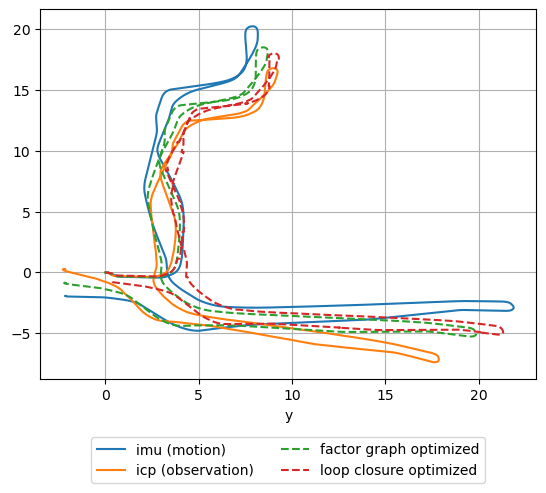
\includegraphics[width=\linewidth]{../img/trj_20.png}
        \caption{trajectory}
        \label{fig:trj_20}
    \end{subfigure}
    \hfill
    \begin{subfigure}{0.24\textwidth}
        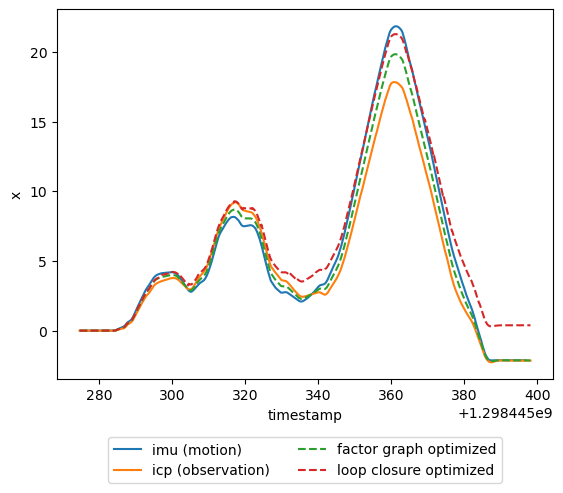
\includegraphics[width=\linewidth]{../img/trj_20_x.png}
        \caption{trajectory x-t}
        \label{fig:trj_20_x}
    \end{subfigure}
    \hfill
    \begin{subfigure}{0.24\textwidth}
        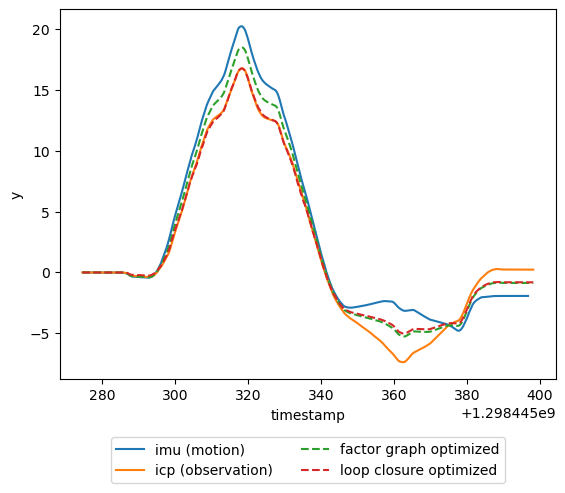
\includegraphics[width=\linewidth]{../img/trj_20_y.png}
        \caption{trajectory y-t}
        \label{fig:trj_20_y}
    \end{subfigure}
    \hfill
    \begin{subfigure}{0.24\textwidth}
        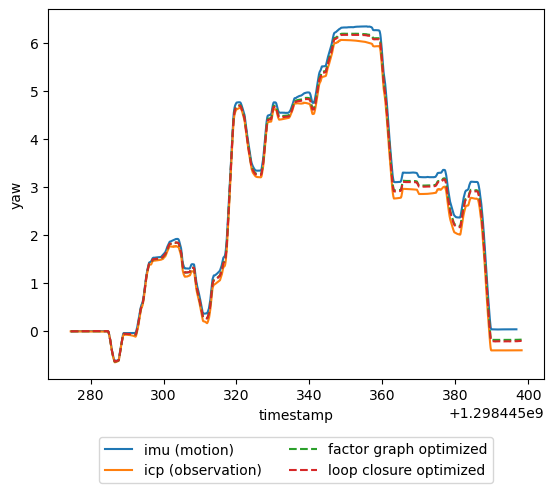
\includegraphics[width=\linewidth]{../img/trj_20_yaw.png}
        \caption{trajectory yaw-t}
        \label{fig:trj_20_yaw}
    \end{subfigure}
    
    % Second row
    \begin{subfigure}{0.24\textwidth}
        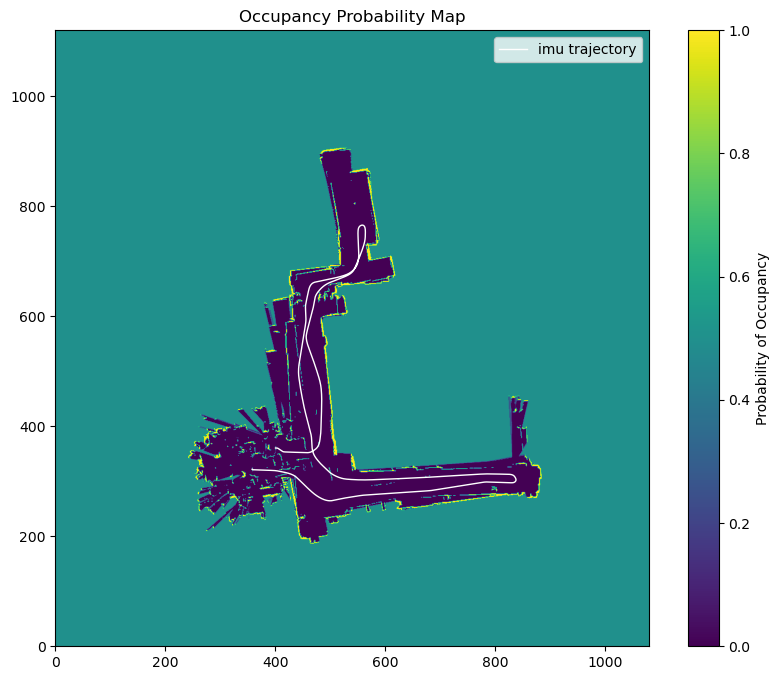
\includegraphics[width=\linewidth]{../img/omap_20_imu.png}
        \caption{occupancy map (motion)}
        \label{fig:omap_20_imu}
    \end{subfigure}
    \hfill
    \begin{subfigure}{0.24\textwidth}
        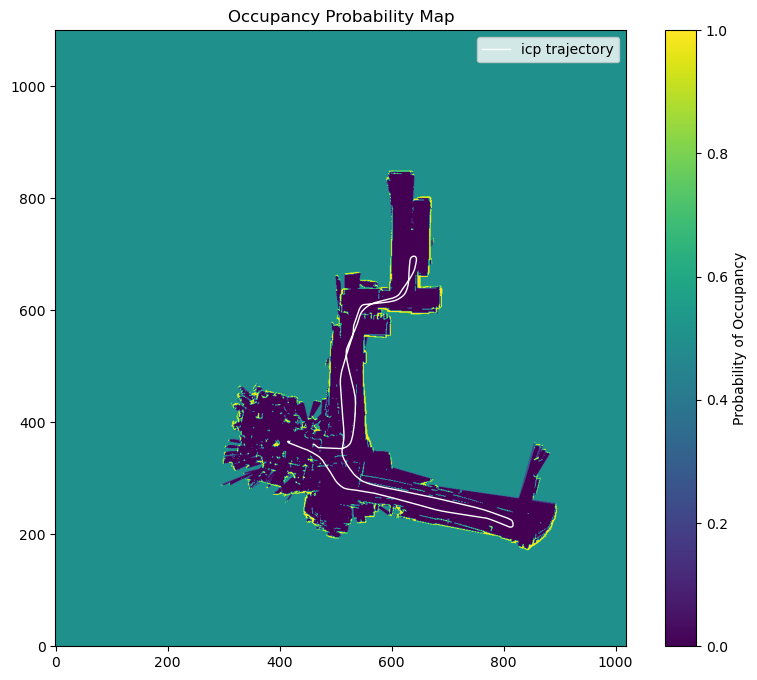
\includegraphics[width=\linewidth]{../img/omap_20_icp.png}
        \caption{occupancy map (observation)}
        \label{fig:omap_20_icp}
    \end{subfigure}
    \hfill
    \begin{subfigure}{0.24\textwidth}
        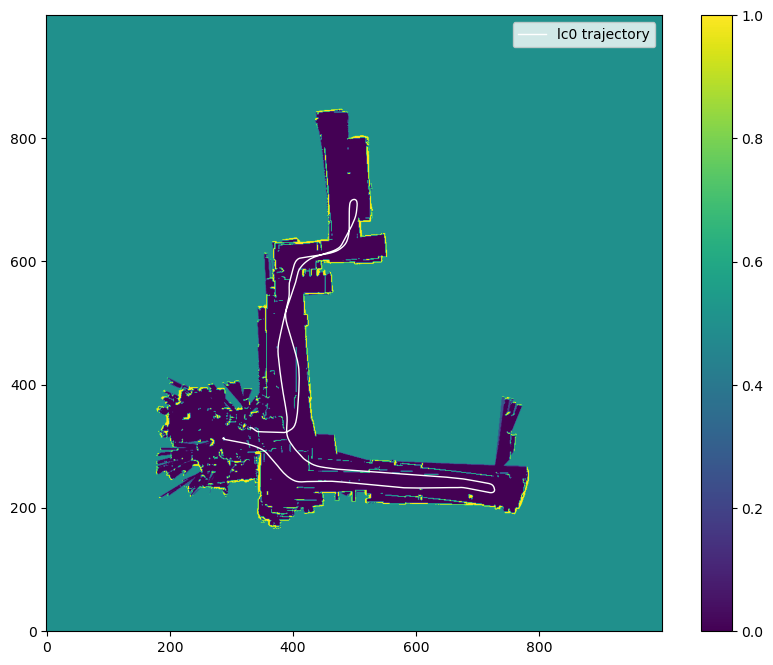
\includegraphics[width=\linewidth]{../img/omap_20_lc0.png}
        \caption{occupancy map (factor graph)}
        \label{fig:omap_20_lc0}
    \end{subfigure}
    \hfill
    \begin{subfigure}{0.24\textwidth}
        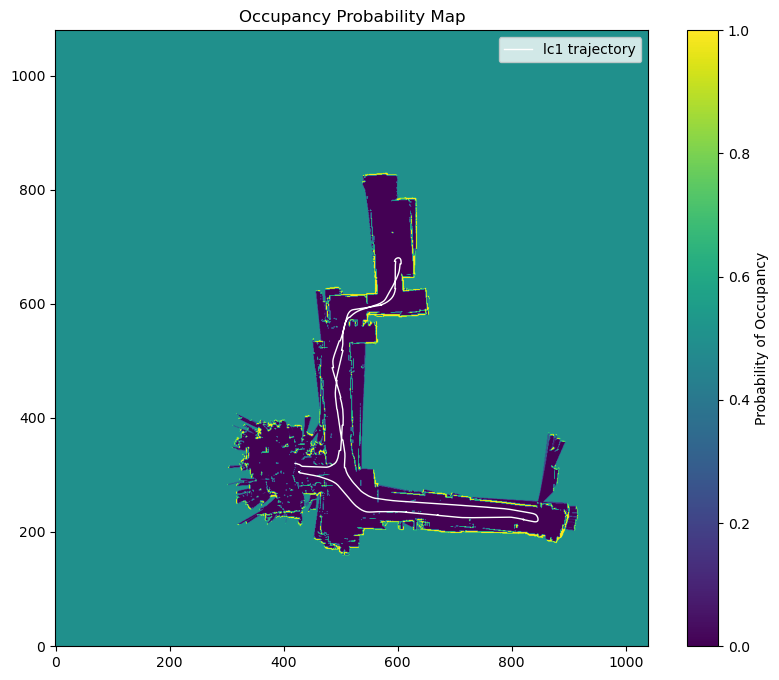
\includegraphics[width=\linewidth]{../img/omap_20_lc1.png}
        \caption{occupancy map (loop closure)}
        \label{fig:omap_20_lc1}
    \end{subfigure}
    
    % Third row
    \begin{subfigure}{0.24\textwidth}
        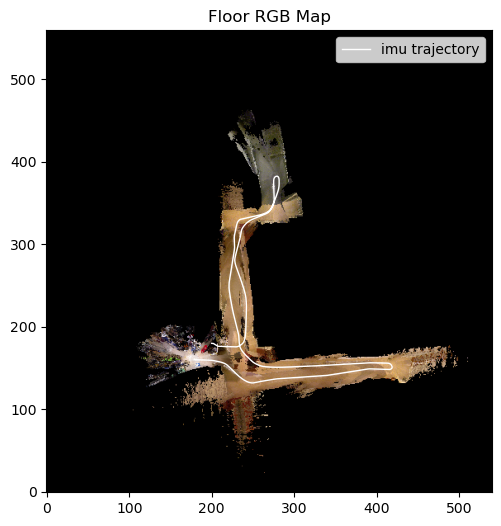
\includegraphics[width=\linewidth]{../img/floormap_20_imu.png}
        \caption{floor map (motion)}
        \label{fig:floormap_20_imu}
    \end{subfigure}
    \hfill
    \begin{subfigure}{0.24\textwidth}
        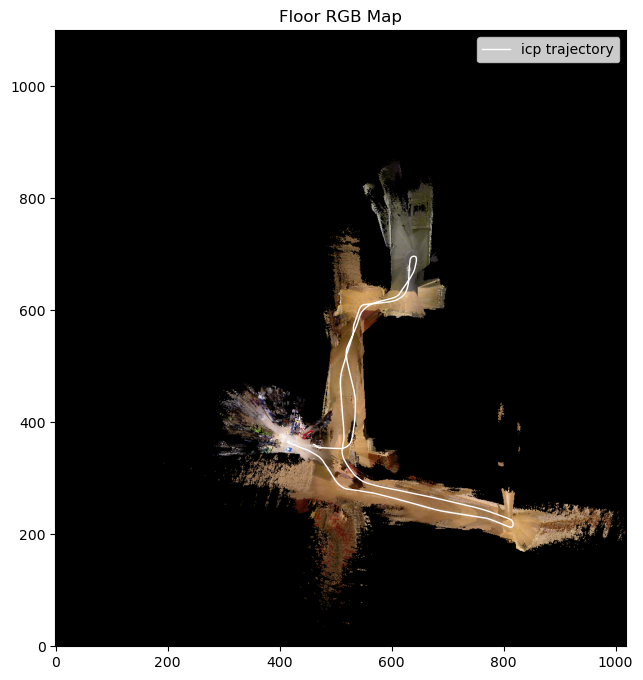
\includegraphics[width=\linewidth]{../img/floormap_20_icp.png}
        \caption{floor map (observation)}
        \label{fig:floormap_20_icp}
    \end{subfigure}
    \hfill
    \begin{subfigure}{0.24\textwidth}
        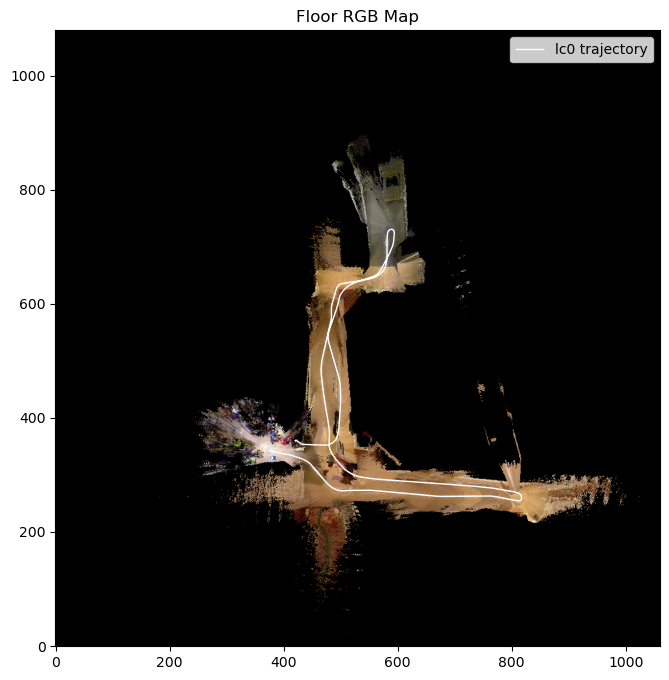
\includegraphics[width=\linewidth]{../img/floormap_20_lc0.png}
        \caption{floor map (factor graph)}
        \label{fig:floormap_20_lc0}
    \end{subfigure}
    \hfill
    \begin{subfigure}{0.24\textwidth}
        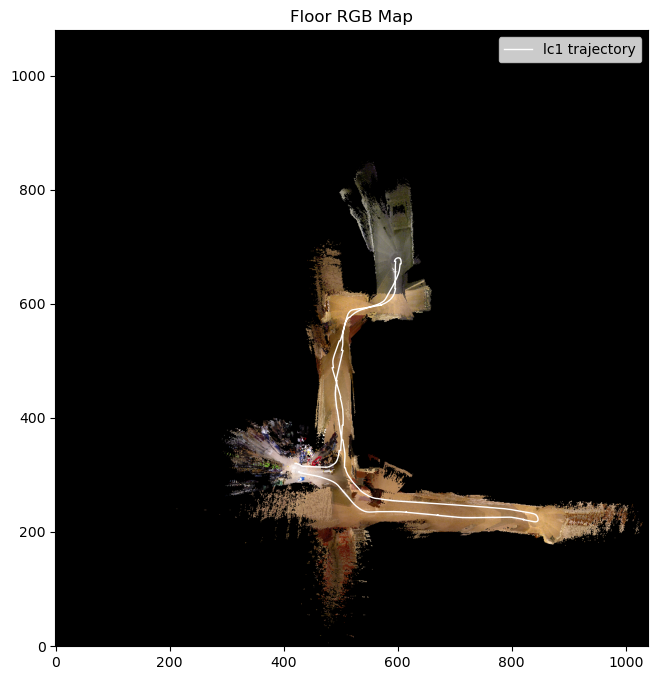
\includegraphics[width=\linewidth]{../img/floormap_20_lc1.png}
        \caption{floor map (loop closure)}
        \label{fig:floormap_20_lc1}
    \end{subfigure}
    
    \caption{dataset 20 results}
    \label{fig:composite}
\end{figure*}



$\{dataset 20, dataset 21\}\times{}$

\subsection{trajectory}

\subsection{occupancy map}

\subsection{floor map}

\appendix
\subsection{ICP warm up}

\subsection{proportion ICP improvement}


\subsection{3D texture mapping}
https://youtu.be/yPtubAjLYnc




\end{document}
